
Alcune informazioni specifiche sono state allegate, approfondite da fonti esterne anche se non specificatamente spiegate all'interno dell'intervista, in modo da sottolineare tutte le procedure e i requisiti da conoscere per poter trattare la vendita alle pubbliche amministrazioni.

%------------------------------------------------
\subsubsection{Prima Intervista} % Sotto_Sotto-Sezione

\medskip

%Per le Interviste questo metodo è ottimo:
%\begin{description}[style=nextline]
%\item[DOMANDA]RISPOSTA  Fare attenzione alle lettere accentate che potrebbero non essere riconosciute
%non scordare di mettere la chiusura di description alla fine   \end{description}

\begin{description}[style=nextline]
    \item[Salve signor Rossi, innanzitutto potrebbe spiegarci esattamente di cosa si occupa la sua azienda]
    La nostra azienda offre servizi e vendita di prodotti sia a privati che a pubbliche amministrazioni. \newline
    La vendita riguarda apparecchiature elettroniche di uso comune legate specialmente all'informatica, dai personal computer ai suoi accessori, dai monitor a componentistica per la gestione di rete, mentre i servizi che offriamo comprendono riparazioni in ufficio ad esempio riparazioni e ripristino di computer, contratti di assistenza "on center", che significa letteralmente sul luogo, cioè contratti di durata solitamente tra i quattro mesi e l'anno, per i quali il cliente paga una quota prestabilita per ricevere assistenza in tempi relativamente brevi, e infine assistenze a chiamata, che comprendono installazioni di apparecchiature elettroniche, come ad esempio la configurazione di computer di laboratori informatici nelle scuole, che è un servizio offerto appunto a delle pubbliche amministrazioni.

    \item[Ci interessa particolarmente la vendita alle pubbliche amministrazioni, ci potrebbe spiegare nello specifico come funziona?]
    Per questioni burocratiche le pubbliche amministrazioni devono redigere delle gare pubbliche effettuando le cosiddette "richieste di offerta" sul mercato elettronico delle pubbliche amministrazioni chiamato MEPA.\newline
    Qui si trovano le richieste di offerta, l'azienda partecipa pubblicamente a queste gare, e poi in base all'esito della gara si può stipulare o meno il contratto.\newline
    C'è anche la possibilità per un istituto statale di fare una trattativa diretta con una particolare azienda abilitata sul MEPA senza la necessità di passare per una gara pubblica.

    \item[Quindi una volta che la vostra azienda partecipa ad una gara qual è l'iter effettivo di vendita e spedizione?]
    Per poter partecipare alla gara si accettano tutte le richieste fatte nello specifico sia che riguardino i prodotti o questioni di carattere legale come ad esempio la garanzia. Quello che manca a questo punto è proprio fare un ordine del prodotto dal fornitore per poi spedirlo oppure erogare direttamente il servizio richiesto. Nel caso di servizio esso viene erogato immediatamente mentre per un ordine i tempi di attesa sono quelli di spedizione del prodotto da parte del fornitore. La vittoria della gara di per se consiste nella firma del contratto.

	\item[Perciò la vendita ad una pubblica amministrazione come si differenzia da una vendita ai privati?]
	Ovviamente la differenza sta nelle modalità con cui le pubbliche amministrazioni acquistano un prodotto, infatti non è il cliente ad andare dal venditore, ma potremmo dire che sono i fornitori che vanno dal cliente. In più da parte del venditore ci deve essere la possibilità, nonchè la volontà, di rispondere ad una gara nei termini da essa richiesti.\newline
	Nella realtà c'è poi il problema della limitatezza della disponibilità dei prodotti richiesti, in quanto il fornitore può non avere la disponibilità necessaria per rispondere alla richiesta della gara.
	In particolare nelle trattative dirette dove la richiesta è diretta. In questo caso sta a noi rivolgerci ai fornitori per poter trovare una soluzione in modo da accettare la richiesta.
	In alcune gare ad esempio viene richiesto specificatamente un prodotto con il suo codice prodotto, bisogna quindi rispondere ad una richiesta molto specifica, in altri casi viene chiesto un prodotto con certe caratteristiche.

	\item[Ed il fatto che sia il venditore che debba adattarsi a quella che è la richiesta del cliente quali ripercussioni ha sul business? Le pubbliche amministrazioni hanno delle specie di convenzioni?]
	Ci sarebbe una sezione del MePA dedicata alle convenzioni, ma l'azienda non aderisce. Comunque le gare hanno un tetto massimo di spesa che influenza le proposte di offerta. Collegandosi al come questo impatta sull'azienda, ciò implica che talvolta si abbassino i propri margini di guadagno per aggiudicarsi una gara.\newline
	I prezzi sono in generale imposti dal mercato in quanto spesso il metodo di giudizio per aggiudicarsi una gara è proprio chi fa il prezzo minore.\newline
	Noi nei cataloghi abbiamo il prezzo di vendita del fornitore, il margine di guadagno viene deciso a posteriori durante la partecipazione alla gara.
	Di solito si tiene una quota percentuale fissa guadagno del 10\% però se con questa percentuale si sfora il tetto massimo può avere senso abbassare la quota per entrare nella gara e vincere.\newline
	Questa tipo di operazione ha senso su vendite più grosse, in quanto il guadagno è inferiore ma su volumi maggiori. Per un computer da 300 euro invece, il 10\% è 30, se 10\% è troppo non lo vendo, non conviene venderlo a meno.


	\item[A proposito di cataloghi, con i fornitori quali rapporti ci sono?]
	La realtà del rapporto con i fornitori è che quando effettuiamo un acquisto, noi paghiamo le spese di spedizione, quindi con i fornitori non c'è un accordo fisso, e quindi il costo delle spedizioni deve essere considerato durante la partecipazione ad una gara, ed è uno dei costi peggiori da tenere in considerazione, ma va calcolato con delle tabelle che può fornire il fornitore in base a vari fattori.
	Noi comunque per semplicità e per evitare di incadere in disagi di questo tipo non vendiamo alle isole, soprattutto per questi costi maggiorati di spedizione.

	\item[Perciò questi cataloghi da cui voi scegliete i prodotti da vendere li fornisce il fornitore?]
	Sì, esatto. I prodotti che noi vendiamo sono quelli che hanno i fornitori, quindi il nostro modello di business è il dropshipping, signfica non abbiamo un magazzino, se la richiesta non può essere soddisfatta dal fornitore rispondiamo di no, specie per le richieste dirette, altrimenti non partecipiamo proprio alla gara.\newline
	Non c'è per forza un rapporto diretto con il fornitore. Per le richieste generiche abbiamo dei cataloghi, quindi non viene sempre contattato, ci basiamo su quello come database, che viene aggiornato una volta al mese, è in formato digitale, fondamentalmente ci viene fornita una nuova tabella excel mensilmente.

	\item[Molto bene, voi offrite servizi oltre che prodotti. Nelle gare essi in che forma vengono descritti e come vengono valutati?]
	Le richieste di servizi sono molto generiche, i servizi sono richiesti con una descrizione generica della prestazione. Da parte nostra bisogna stimare il loro costo, il che non è una cosa banale.\newline Solitamente non si lavora ad ore ma si lavora per tipo di lavoro svolto, quindi è difficile standardizzare il costo della prestazione. Può essere semplice definire un costo per certi servizi, come ad esempio la formattazione di un computer, che richiede generalmente un tempo standard di lavorazione, ma risulta molto più difficile rispondere alla richiesta di installazione di una rete wifi, per cui il tempo di lavoro varia in base alla dimensione, alla struttura ed altri fattori.\newline Sarebbe molto interessante trovare un sistema per standardizzare in qualche modo questo processo.

	\item[Ottimo quindi a livello operativo sarebbe utile intanto una registrazione delle gare?]
	Sarebbe sicuramente utile avere una tabella delle gare a cui abbiamo partecipato, con indicato se la gara è stata vinta o persa.\newline
	Nel caso sia persa sarebbe buono poter avere anche il prezzo del dato di chi ha vinto la gara a scopo statistico. In questo modo sarebbe utile effettuato delle analisi statistiche di mercato per quanto  riguarda i competitor e i prezzi con cui si sono aggiudicati le gare.

	\item[Il risultato della gara perciò è pubblico e chiunque può vederne il risultato?]
	Sì assolutamente sul sito delle gare è possibile visionare le offerte dei concorrenti e l'aggiudicatario definitivo.
	Quindi è possibile tenere traccia di tutto lo svolgimento della gara.

	\item[Quindi se abbiamo capito bene, adesso è tutto gestito a mano tramite tabelle excel. Vi è innanzitutto la necessità di implementare una base di dati che tenga traccia di tutte le informazioni.]
	Sì esattamente ora è gestito tutto a mano, sarebbe già molto utile implementare un sistema informativo in cui inserire tutti i dati.

	\item[Molto bene allora tenendo conto di quanto detto abbiamo una serie di elementi che potrebbero essere gestiti dal sistema informativo. Prima di tutto le gare come appena detto. All'inizio parlavamo di contratti di diverso tipo stipulati. Questi sono registrabili?]
	Certamente i contratti hanno un modello standard, possono essere riportati.

	\item[Bene, inoltre legati ai contratti ci sono anche le trattative dirette. Abbiamo parlato dei fornitori, quindi dei loro cataloghi, e di conseguenza degli ordini che vengono effettuati, tutto ciò sarebbe sicuramente da registrare.]
	Sarebbe ottimo tener traccia di tutti questi dati.

	\item[Ovviamente come avevamo già accennato sarebbe buono sfruttare questi dati a fini statistici per analizzare le gare vinte e perse e quali sono i prodotti più venduti. Sarebbe interessante sviluppare un sistema che riesca a fornire le soluzioni ottimali per rispondere alle richieste delle gare, tenendo conto dei margini e dei volumi di vendita.]
	Wow sarebbe un sistema utilissimo se può essere realizzato, ci semplificherebbe molto il lavoro!

	\item[Non ci dimentichiamo della gestione dei clienti, intesi come pubbliche amministrazioni che acquistano da voi, le fatture associate agli ordini e i costi di spedizione, tutto ciò può essere registrato nel sistema informativo. Ci dimentichiamo qualcosa?]
	Sembrano esserci molte informazioni. Sarebbe interessante se fosse possibile consultare questi dati, in base all'andamento di certi periodi dell'anno, calcolare il bilancio magari ad una certa data. E poi magari tenere traccia dei pagamenti effettuati e ricevuti, in modo da tener sotto controllo le varie scadenze.

	\item[Certamente possiamo implementare queste soluzioni. Non mi viene in mente altro al momento. Potremmo cominciare a progettare il sistema, e nel caso in cui si palesino dubbi riguardo il funzionamento dei vari apparati potremmo sentirci di nuovo per eventuali chiarimenti.]
	Sicuramente ragazzi vi ringrazio molto, sono disponibile per qualsiasi chiarimento, vi auguro buona giornata, a risentirci.


    \end{description}

%------------------------------------------------
\subsubsection{Raccolta informazioni (modulistica)}
Il titolare dell'azienda Rimini Service ci ha fornito una serie di documenti contenenti informazioni utili ai nostri scopi. Sono mostrati qui di seguito:

\includepdf[]{./pdf/moduli2.pdf}
\includepdf[]{./pdf/moduli.pdf}

%-------------------------------------------------------------------------
\subsubsection{Analisi delle Azioni e dei Processi Interni}

Partendo dalle interviste e utlizzando i documenti forniti, abbiamo voluto organizzare le informazioni in uno schema dei processi interni, per poter avere una miglior comprensione del flusso di operazioni interne all'azienda. Abbiamo costruito uno schema piuttosto informale, in cui sono presenti ridondanze che verranno analizzate in seguito. E' possibile osservare il flusso di operazioni partendo da un contatto tra cliente e azienda, che può avvenire in 3 modi: un privato contatta l'azienda, una pubblica amministrazione contatta l'azienda attraverso una trattativa diretta, oppure l'azienda si mette in contatto con una pubblica amministrazione attraverso una gara pubblica.\newline
Segue lo schema:\newline\newline\newline\newline\newline

\noindent\makebox[\textwidth]{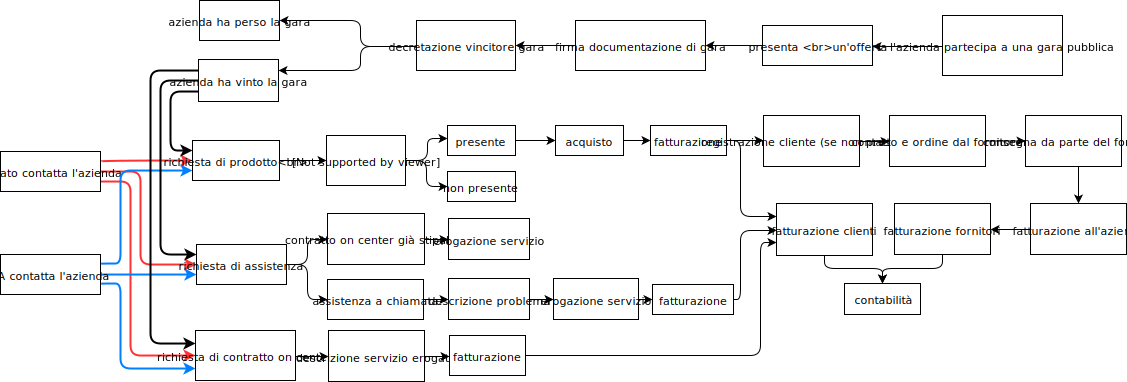
\includegraphics[width=\paperwidth-1cm, trim={0 8cm 0 0}, clip]{./immagini/processi_interni.pdf}}


% \newpage
%
% \begin{landscape} %inizia un foglio landscape
%
%
% %include un file pdf che contiene lo schema ruotato e dimensionato correttamente
% 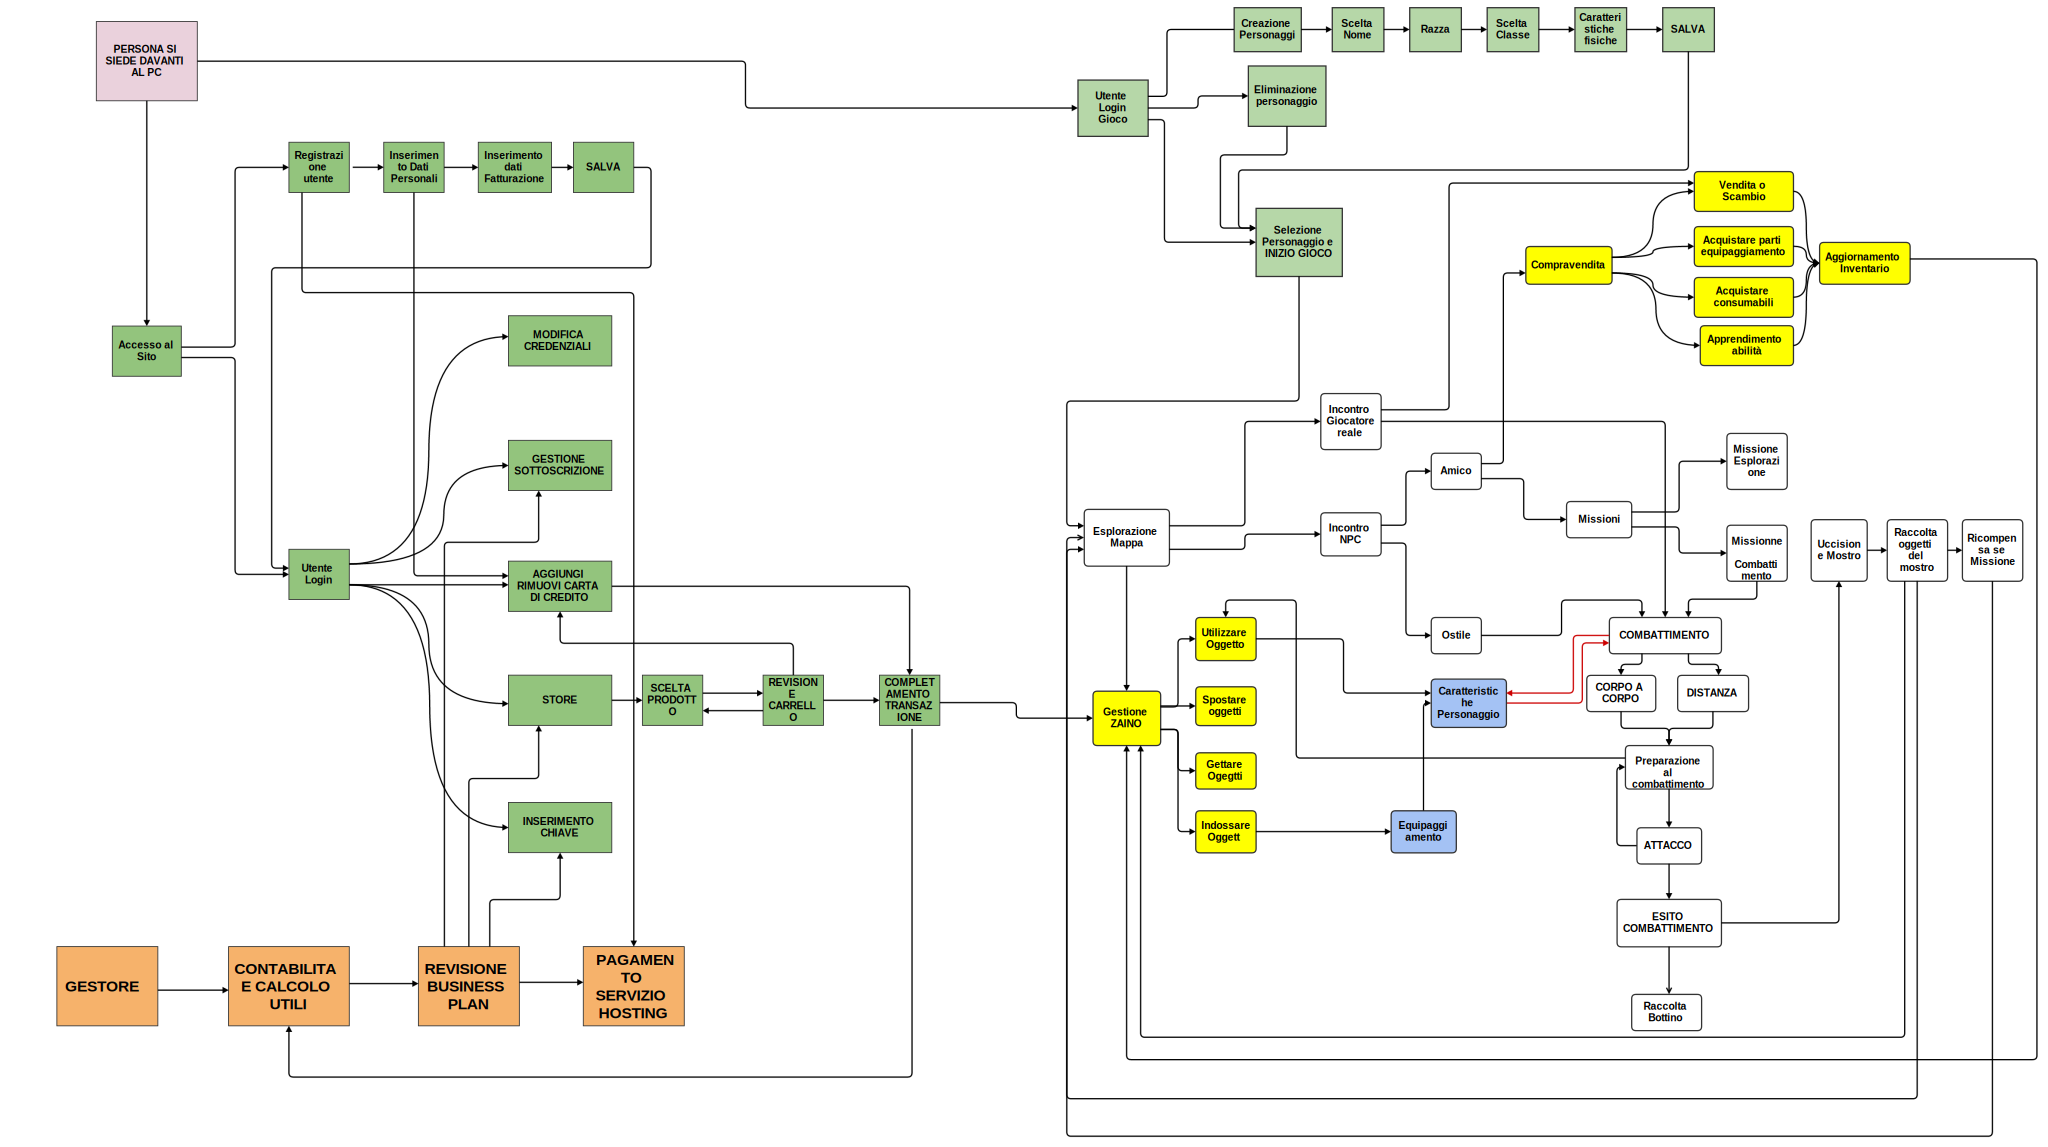
\includepdf[width=270mm, height=210mm, angle=90, keepaspectratio]{./pdf/sprocint.pdf}
%
% \end{landscape}
